% Options for packages loaded elsewhere
\PassOptionsToPackage{unicode}{hyperref}
\PassOptionsToPackage{hyphens}{url}
\PassOptionsToPackage{dvipsnames,svgnames,x11names}{xcolor}
%
\documentclass[
  letterpaper,
  DIV=11,
  numbers=noendperiod]{scrartcl}

\usepackage{amsmath,amssymb}
\usepackage{iftex}
\ifPDFTeX
  \usepackage[T1]{fontenc}
  \usepackage[utf8]{inputenc}
  \usepackage{textcomp} % provide euro and other symbols
\else % if luatex or xetex
  \usepackage{unicode-math}
  \defaultfontfeatures{Scale=MatchLowercase}
  \defaultfontfeatures[\rmfamily]{Ligatures=TeX,Scale=1}
\fi
\usepackage{lmodern}
\ifPDFTeX\else  
    % xetex/luatex font selection
\fi
% Use upquote if available, for straight quotes in verbatim environments
\IfFileExists{upquote.sty}{\usepackage{upquote}}{}
\IfFileExists{microtype.sty}{% use microtype if available
  \usepackage[]{microtype}
  \UseMicrotypeSet[protrusion]{basicmath} % disable protrusion for tt fonts
}{}
\makeatletter
\@ifundefined{KOMAClassName}{% if non-KOMA class
  \IfFileExists{parskip.sty}{%
    \usepackage{parskip}
  }{% else
    \setlength{\parindent}{0pt}
    \setlength{\parskip}{6pt plus 2pt minus 1pt}}
}{% if KOMA class
  \KOMAoptions{parskip=half}}
\makeatother
\usepackage{xcolor}
\setlength{\emergencystretch}{3em} % prevent overfull lines
\setcounter{secnumdepth}{5}
% Make \paragraph and \subparagraph free-standing
\makeatletter
\ifx\paragraph\undefined\else
  \let\oldparagraph\paragraph
  \renewcommand{\paragraph}{
    \@ifstar
      \xxxParagraphStar
      \xxxParagraphNoStar
  }
  \newcommand{\xxxParagraphStar}[1]{\oldparagraph*{#1}\mbox{}}
  \newcommand{\xxxParagraphNoStar}[1]{\oldparagraph{#1}\mbox{}}
\fi
\ifx\subparagraph\undefined\else
  \let\oldsubparagraph\subparagraph
  \renewcommand{\subparagraph}{
    \@ifstar
      \xxxSubParagraphStar
      \xxxSubParagraphNoStar
  }
  \newcommand{\xxxSubParagraphStar}[1]{\oldsubparagraph*{#1}\mbox{}}
  \newcommand{\xxxSubParagraphNoStar}[1]{\oldsubparagraph{#1}\mbox{}}
\fi
\makeatother


\providecommand{\tightlist}{%
  \setlength{\itemsep}{0pt}\setlength{\parskip}{0pt}}\usepackage{longtable,booktabs,array}
\usepackage{calc} % for calculating minipage widths
% Correct order of tables after \paragraph or \subparagraph
\usepackage{etoolbox}
\makeatletter
\patchcmd\longtable{\par}{\if@noskipsec\mbox{}\fi\par}{}{}
\makeatother
% Allow footnotes in longtable head/foot
\IfFileExists{footnotehyper.sty}{\usepackage{footnotehyper}}{\usepackage{footnote}}
\makesavenoteenv{longtable}
\usepackage{graphicx}
\makeatletter
\newsavebox\pandoc@box
\newcommand*\pandocbounded[1]{% scales image to fit in text height/width
  \sbox\pandoc@box{#1}%
  \Gscale@div\@tempa{\textheight}{\dimexpr\ht\pandoc@box+\dp\pandoc@box\relax}%
  \Gscale@div\@tempb{\linewidth}{\wd\pandoc@box}%
  \ifdim\@tempb\p@<\@tempa\p@\let\@tempa\@tempb\fi% select the smaller of both
  \ifdim\@tempa\p@<\p@\scalebox{\@tempa}{\usebox\pandoc@box}%
  \else\usebox{\pandoc@box}%
  \fi%
}
% Set default figure placement to htbp
\def\fps@figure{htbp}
\makeatother

\KOMAoption{captions}{tableheading}
\makeatletter
\@ifpackageloaded{caption}{}{\usepackage{caption}}
\AtBeginDocument{%
\ifdefined\contentsname
  \renewcommand*\contentsname{Table of contents}
\else
  \newcommand\contentsname{Table of contents}
\fi
\ifdefined\listfigurename
  \renewcommand*\listfigurename{List of Figures}
\else
  \newcommand\listfigurename{List of Figures}
\fi
\ifdefined\listtablename
  \renewcommand*\listtablename{List of Tables}
\else
  \newcommand\listtablename{List of Tables}
\fi
\ifdefined\figurename
  \renewcommand*\figurename{Figure}
\else
  \newcommand\figurename{Figure}
\fi
\ifdefined\tablename
  \renewcommand*\tablename{Table}
\else
  \newcommand\tablename{Table}
\fi
}
\@ifpackageloaded{float}{}{\usepackage{float}}
\floatstyle{ruled}
\@ifundefined{c@chapter}{\newfloat{codelisting}{h}{lop}}{\newfloat{codelisting}{h}{lop}[chapter]}
\floatname{codelisting}{Listing}
\newcommand*\listoflistings{\listof{codelisting}{List of Listings}}
\makeatother
\makeatletter
\makeatother
\makeatletter
\@ifpackageloaded{caption}{}{\usepackage{caption}}
\@ifpackageloaded{subcaption}{}{\usepackage{subcaption}}
\makeatother

\usepackage{bookmark}

\IfFileExists{xurl.sty}{\usepackage{xurl}}{} % add URL line breaks if available
\urlstyle{same} % disable monospaced font for URLs
\hypersetup{
  pdftitle={The ``A'' of Statistics II (and III)},
  pdfauthor={Bryan Mui - UID 506021334},
  colorlinks=true,
  linkcolor={blue},
  filecolor={Maroon},
  citecolor={Blue},
  urlcolor={Blue},
  pdfcreator={LaTeX via pandoc}}


\title{The ``A'' of Statistics II (and III)}
\usepackage{etoolbox}
\makeatletter
\providecommand{\subtitle}[1]{% add subtitle to \maketitle
  \apptocmd{\@title}{\par {\large #1 \par}}{}{}
}
\makeatother
\subtitle{Mini Workshop}
\author{Bryan Mui - UID 506021334}
\date{January 25, 2025}

\begin{document}
\maketitle


\section{Introduction}\label{introduction}

We assume you have already viewed a ``client interview'' (or, client
discovery) video featuring Professor Esfandiari and Dr.~Rootman.

This assignment is an individual submission which counts for two
individual assignments. For this part, please read Ruland's First and
Second Questions in the book ``Guide for the New Statistical
Consultant''.

\section{Your Work}\label{your-work}

Make sure to include your name on your submission. Your student ID is
not necessary.

Please submit answers as PDF output (include the scripts that produced
them - Quarto or LaTeX preferred, you can modify the files that produced
this document)to the following prompts:

\subsection{Imagine yourself as Dr.~Rootman. Formulate responses to the
following three
questions.}\label{imagine-yourself-as-dr.-rootman.-formulate-responses-to-the-following-three-questions.}

\begin{enumerate}
\def\labelenumi{\arabic{enumi}.}
\tightlist
\item
  What does one, complete, single observation look like?
\end{enumerate}

\begin{itemize}
\tightlist
\item
  \textbf{One, complete observation would have the picture's flash
  position and lightning effect, along with the rating of that person's
  attractiveness}
\end{itemize}

\begin{enumerate}
\def\labelenumi{\arabic{enumi}.}
\setcounter{enumi}{1}
\tightlist
\item
  If you measure this again, will you get the same answer?\\
\end{enumerate}

\begin{itemize}
\tightlist
\item
  \textbf{No, because every person's attractiveness is subjective, so
  the results of the analysis might be different if the experiment was
  repeated}
\end{itemize}

\begin{enumerate}
\def\labelenumi{\arabic{enumi}.}
\setcounter{enumi}{2}
\tightlist
\item
  If we can answer your research questions, what will you do next?\\
\end{enumerate}

\begin{itemize}
\tightlist
\item
  \textbf{We would change the way we take photos for before/after to
  improve desirability for plastic surgery, so people would support our
  business}
\end{itemize}

\subsection{Analysis}\label{analysis}

You have been given access to the original Rootman data (it's the Excel
file found in the link on the assignment page). You have also been given
a modified form of the original data called ``lighting\_tall.tsv''.
Please use any of the formats or your own modified form of the data to
produce two results (whatever language you wish to use, e.g., Python)

\begin{enumerate}
\def\labelenumi{\arabic{enumi}.}
\tightlist
\item
  One data visualization
\end{enumerate}

\pandocbounded{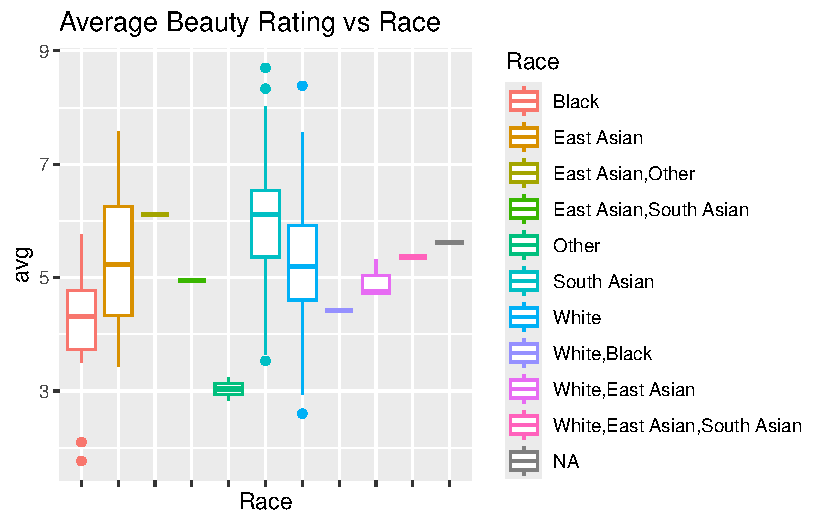
\includegraphics[keepaspectratio]{_yourKit_01_files/figure-pdf/unnamed-chunk-3-1.pdf}}

\begin{enumerate}
\def\labelenumi{\arabic{enumi}.}
\setcounter{enumi}{1}
\tightlist
\item
  One table of some sort (could be simple counts could be more complex
  like model output)
\end{enumerate}

\begin{verbatim}

Call:
lm(formula = avg ~ as.numeric(Age) + Sex, data = data)

Residuals:
    Min      1Q  Median      3Q     Max 
-3.4132 -0.6377  0.0044  0.7483  3.5505 

Coefficients:
                Estimate Std. Error t value Pr(>|t|)    
(Intercept)     5.050835   0.401958  12.566   <2e-16 ***
as.numeric(Age) 0.003794   0.008751   0.434    0.665    
SexMale         0.219558   0.182310   1.204    0.230    
---
Signif. codes:  0 '***' 0.001 '**' 0.01 '*' 0.05 '.' 0.1 ' ' 1

Residual standard error: 1.171 on 197 degrees of freedom
Multiple R-squared:  0.007412,  Adjusted R-squared:  -0.002665 
F-statistic: 0.7355 on 2 and 197 DF,  p-value: 0.4806
\end{verbatim}

These should fit into the context of the problem that Dr.~Rootman wass
seeking to solve. You could look at the graduate lab example that can be
found with the Ruland reading as an encouragement.

\begin{enumerate}
\def\labelenumi{\arabic{enumi}.}
\setcounter{enumi}{2}
\tightlist
\item
  Please record yourself (like your UCLA Story video) telling us a story
  about either your visualization OR your table (what is this result
  communicating to you and please communicate it to your viewer). Not
  both, choose one. The story might be really short (e.g., ``this is a
  histogram of score'')
\end{enumerate}

\begin{itemize}
\tightlist
\item
  \textbf{Video attached with submission}*
\end{itemize}

\section{What to turn in}\label{what-to-turn-in}

\begin{enumerate}
\def\labelenumi{\arabic{enumi}.}
\tightlist
\item
  A single PDF with your name somewhere answering the questions and
  providing either a visualization or a table. The PDF help your tell
  the story you want to tell (writing things out will be helpful before
  having to talk about the result on video).
\item
  A video recording (.mp4 or .mov work best)
\item
  The associated code that produced the PDF and the analysis
  (visualization code or table code). Quarto or \LaTeX~or RMarkdown is
  preferred, but it is OK if you used something else, just include it as
  part of the submission (like a link).
\item
  This is due before the next meeting when we will see the team's
  answer.
\end{enumerate}

\section{Reminders}\label{reminders}

\begin{enumerate}
\def\labelenumi{\arabic{enumi}.}
\tightlist
\item
  It's the story that is most important, the graphic and the table only
  lend support.
\item
  Your PDF does not need to be very long, a page or two is about all you
  need.
\item
  Your recording does not need to be very long, less than minute, but no
  penalties if it runs long.
\item
  It's OK to turn this in late, just upload it as a comment but
  remember, once I finish grading, it's a zero because reopening a
  completed assessment is a headache\ldots{}
\end{enumerate}




\end{document}
